\chapter{Diseño de la arquitectura}
\label{chap:arquitectura}

\section{Visión general}
\label{sec:vision-general-arquitectura}

La arquitectura global se basa en una API REST monolítica, \gls{stateless} y contenerizada. El cliente accede al sistema a través de un endpoint público gestionado por un \acrshort{alb}, mientras que la ejecución de la aplicación y la base de datos permanecen en subredes privadas. Esta separación permite exponer únicamente el balanceador de carga y mantener PostgreSQL aislado de Internet.

En local, el sistema se ejecuta con Docker Compose, levantando la API y PostgreSQL. En AWS, la API se publica como imagen Docker en ECR y se ejecuta en ECS Fargate. RDS PostgreSQL actúa como almacén persistente. Route 53 resuelve el dominio \endpoint{api.dev.transitops.net}, ACM emite el certificado \acrshort{tls} y el \acrshort{alb} centraliza el tráfico público. La validación cloud admite un fallback HTTP mediante el \acrshort{dns} técnico del \acrshort{alb} cuando se recrea el entorno antes de completar la delegación DNS, pero la configuración objetivo de Terraform activa \acrshort{https} y redirección de HTTP a \acrshort{https}.

La infraestructura se define mediante Terraform, con módulos reutilizables para red, registro de contenedores, base de datos, configuración, observabilidad y runtime de contenedores. Esta decisión permite reproducir el entorno, revisar los cambios de infraestructura como parte del repositorio y destruir el entorno \texttt{dev} tras las validaciones para controlar el coste.

\section{Arquitectura lógica del backend}
\label{sec:arquitectura-logica-backend}

El backend se organiza como una solución .NET deliberadamente simple con dos proyectos: \path{TransitOps.Api} y \path{TransitOps.Tests}. Dentro de la API se distinguen responsabilidades por carpetas:

\begin{itemize}
  \item \texttt{Controllers}: puntos de entrada HTTP versionados.
  \item \texttt{Contracts}: objetos de petición y respuesta expuestos por la API.
  \item \texttt{Application}: servicios de aplicación que contienen la lógica de casos de uso.
  \item \texttt{Domain}: entidades y enumeraciones del dominio.
  \item \texttt{Infrastructure}: persistencia, configuración EF Core y migraciones.
  \item \texttt{Common}, \texttt{Errors} y \texttt{Middleware}: contrato común de respuestas, errores y tratamiento transversal.
\end{itemize}

No se ha dividido el backend en múltiples proyectos de dominio, aplicación e infraestructura porque el tamaño del sistema no lo justifica. La separación interna por carpetas ofrece suficiente claridad sin añadir coste accidental.

\section{Arquitectura de datos}
\label{sec:arquitectura-datos}

PostgreSQL se utiliza como base de datos principal. El esquema se gestiona mediante migraciones de Entity Framework Core, ubicadas bajo \path{TransitOps.Api/Infrastructure/Persistence/Migrations}. Esta carpeta es la fuente de verdad del esquema, tanto para local como para cloud.

Las entidades principales aplican campos de auditoría y borrado lógico mediante \texttt{deleted\_at}. Por ello, varias restricciones de unicidad se han diseñado para registros activos, permitiendo reutilizar identificadores de negocio cuando un registro anterior ha sido eliminado lógicamente. Este criterio aparece en referencias como matrículas de vehículos, licencias de conductores o referencias de transporte.

Los estados y tipos de evento se almacenan como \texttt{smallint} con restricciones \texttt{check}. Esta solución evita depender de enumerados nativos de PostgreSQL y simplifica la integración con EF Core, manteniendo a la vez validación a nivel de base de datos.

\section{Arquitectura cloud en AWS}
\label{sec:arquitectura-cloud}

La arquitectura cloud desplegable en AWS incluye Route 53, ACM, \acrshort{alb}, \acrshort{ecs} Fargate, \acrshort{ecr}, \acrshort{rds} PostgreSQL, Secrets Manager, \acrshort{ssm} Parameter Store y CloudWatch~\cite{AwsEcsDocs,AwsAlbDocs,AwsRoute53Docs,AwsAcmDocs,AwsRdsDocs,AwsCloudWatchDocs,AwsSecretsManagerDocs,AwsSystemsManagerDocs}.

El entorno \texttt{dev} se despliega en la cuenta AWS \texttt{661000947340}, región \texttt{eu-west-1}. La red está formada por una \acrshort{vpc} con subredes públicas para \acrshort{alb} y NAT, subredes privadas de aplicación para ECS y subredes privadas de datos para RDS. Los grupos de seguridad restringen el flujo a: Internet hacia \acrshort{alb}, \acrshort{alb} hacia ECS y ECS hacia RDS.

La API queda preparada para exponerse como \endpoint{https://api.dev.transitops.net}. En la cuenta objetivo se dispone del dominio \path{transitops.net} y de una hosted zone pública de Route 53; durante Sprint 6 se corrigió la delegación de nameservers para que la validación \acrshort{dns} de ACM fuese visible públicamente. Terraform crea el certificado, los registros de validación, el alias \endpoint{api.dev.transitops.net}, el listener \acrshort{https} y la redirección HTTP a \acrshort{https} cuando \texttt{enable\_https = true}. La base de datos RDS no es pública y solo acepta tráfico PostgreSQL desde el grupo de seguridad de ECS.

\begin{figure}[htbp]
\centering
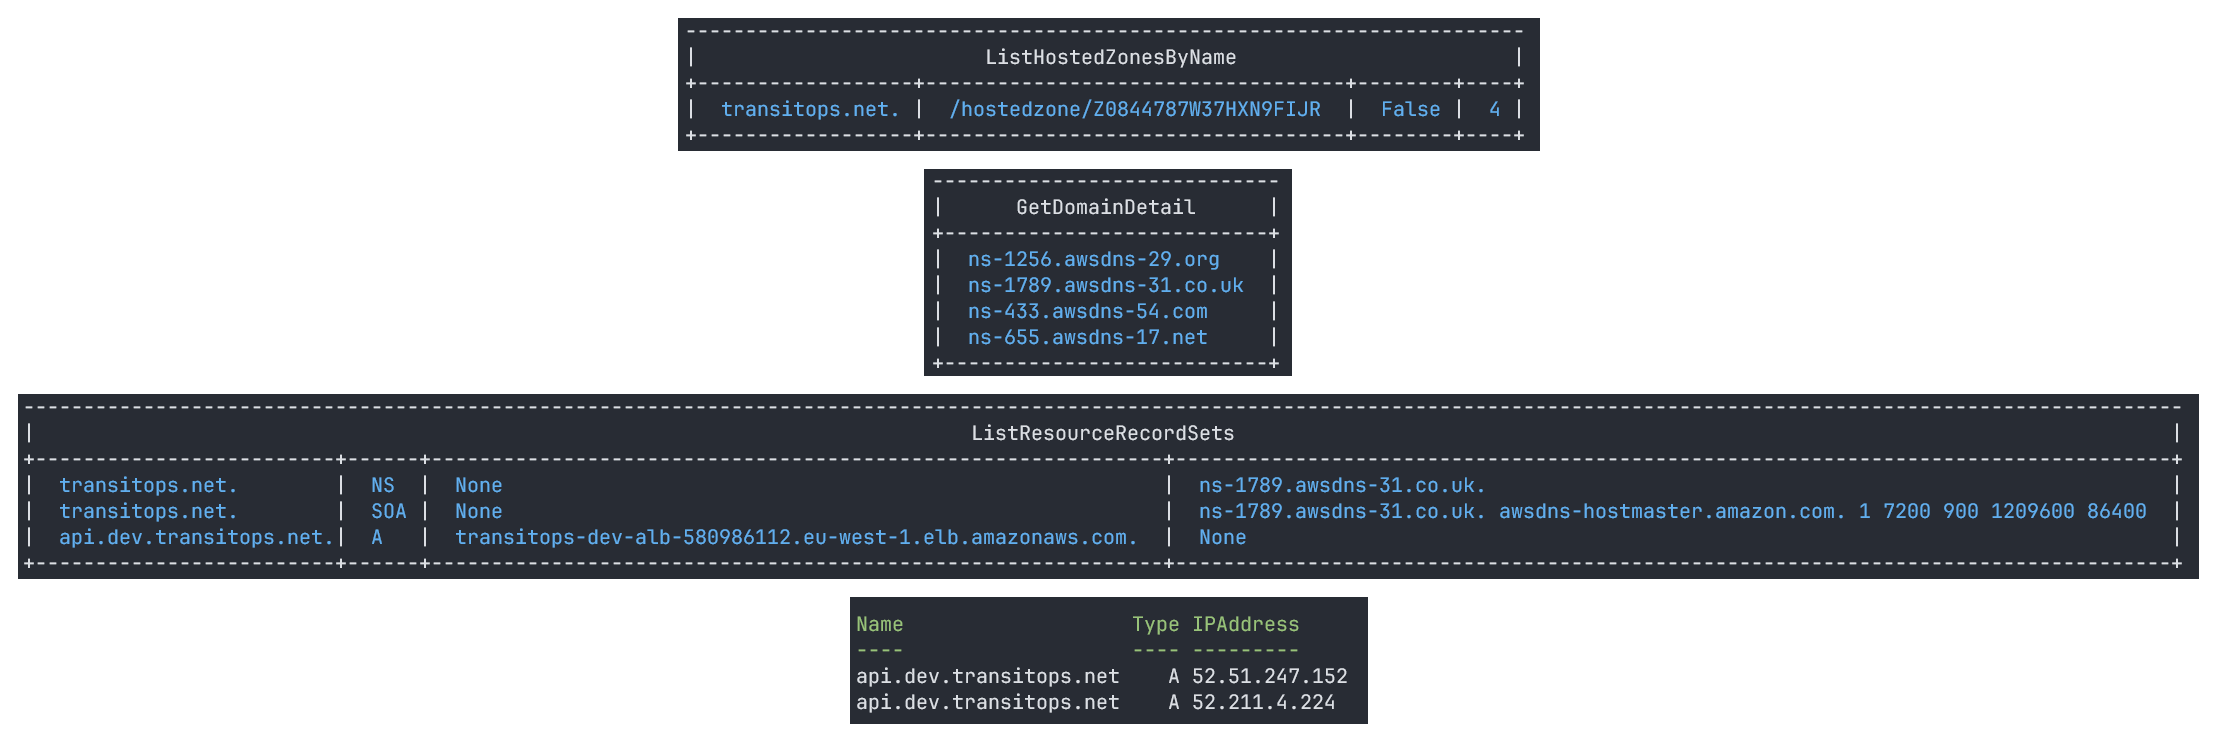
\includegraphics[width=0.92\textwidth]{imaxes/route53-dns-evidence}
\caption{Evidencia DNS para el endpoint de desarrollo.}
\label{fig:route53-dns}
\end{figure}

\section{Decisiones arquitectónicas}
\label{sec:decisiones-arquitectonicas}

Las decisiones arquitectónicas principales han sido:

\begin{itemize}
  \item Monolito modular frente a microservicios: el dominio y el tamaño del trabajo no justifican la complejidad de microservicios, mensajería o orquestación avanzada.
  \item ECS Fargate frente a servidores EC2: Fargate reduce administración de infraestructura y encaja bien con una API stateless contenerizada.
  \item RDS PostgreSQL frente a PostgreSQL autogestionado: RDS simplifica backups, operación y red privada.
  \item Terraform frente a creación manual: la infraestructura queda versionada, reproducible y revisable~\cite{TerraformDocs}.
  \item Secrets Manager y SSM frente a variables hardcodeadas: los secretos no se almacenan en el repositorio y pueden gestionarse de forma separada.
  \item Migraciones como tarea ECS puntual frente a migraciones automáticas en producción: el despliegue gana control explícito y evita que cada arranque web modifique el esquema.
  \item OIDC en GitHub Actions frente a claves AWS persistentes: se reduce el riesgo de credenciales de larga duración.
  \item Observabilidad mínima con CloudWatch frente a plataformas externas: el sprint prioriza logs JSON, correlación, dashboard y alarmas con servicios ya disponibles en AWS, evitando introducir herramientas adicionales antes de que exista una necesidad real.
\end{itemize}

Estas decisiones favorecen una arquitectura pequeña pero defendible, orientada a demostrar operación real en cloud.
